\PassOptionsToPackage{dvipsnames,table}{xcolor}
\documentclass[10pt]{beamer}
\usepackage{Cours}

\begin{document}

\input{\detokenize{/home/fenarius/Travail/Cours/NSITerminale/docs/commun/MacrosCours.tex}}
\setcounter{numchap}{11}
\newcommand{\GR}{\cnum Graphes}

\pythonmode


% Aspect historique, définition
\begin{frame}
	\mframe{\GR}
	\begin{block}{Aspect historique}
		\begin{itemize}
			\item<1-> C'est le mathématicien suisse Leonhard Euler (1707-1783) qui est à l'origine de la création de la théorie des graphes.
			\item<2-> Il en pose les bases en résolvant le problème des 7 ponts de  Königsberg (voir activité) en 1740.
			\item<3-> Les graphes interviennent à présent dans de nombreux problèmes (recherche de chemins, réseau, \dots) en informatique comme en mathématiques.
		\end{itemize}
	\end{block}
	\begin{alertblock}{Définition}
		\onslide<4->{Un \textcolor{red}{graphe} est la donnée :}
		\begin{itemize}
			\item<5->{D'un ensemble de sommet $S$ (on dit aussi noeuds ou points)}
			\item<6->{D'un ensemble d'arêtes $E$, chaque arête étant une paire de sommets}
		\end{itemize}
	\end{alertblock}
\end{frame}

% Premiers exemples
\begin{frame}
	\mframe{\GR}
	\begin{exampleblock}{Exemples}
		\begin{enumerate}
			\item On représente par un graphe un minuscule réseau social de 5 personnes : Amélie, Philippe, John, Brice et Alice. Dessiner ce graphe sachant que Philippe est ami avec tout le monde, Amélie et Alice sont amies de même que Brice et John. Donner l'ensemble des arêtes de ce graphe.
			\item Donner l'ensemble des sommets et des arêtes du graphe suivant :
			      \begin{center}
				      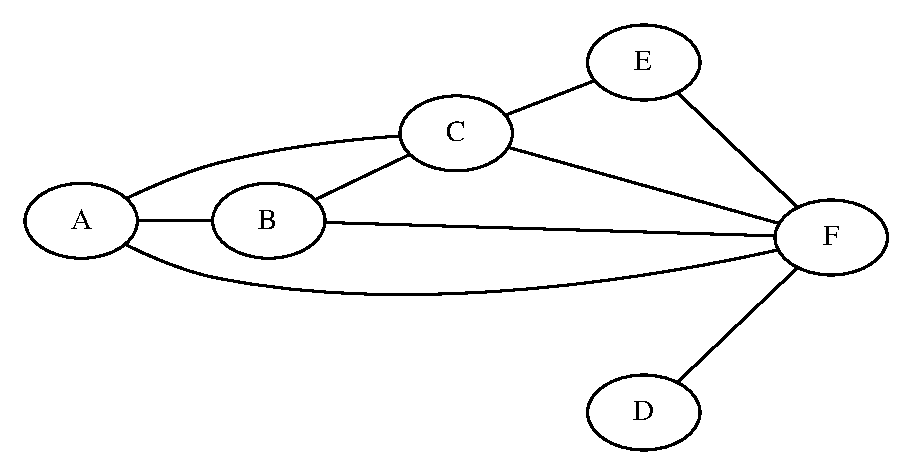
\includegraphics[scale=0.4]{graph1.eps}
			      \end{center}
		\end{enumerate}
	\end{exampleblock}
\end{frame}

% Vocabulaire
\begin{frame}
	\mframe{\GR}
	\begin{block}{Vocabulaire}
		\begin{itemize}
			\item<1-> On dit que deux sommets sont \textcolor{blue}{adjacents} lorsqu'une arête les relie. Les \textcolor{blue}{voisins} d'un sommet sont les sommets adjacents à ce sommet.
			\item<2-> Le \textcolor{blue}{degré (ou ordre) du graphe} est son nombre de sommets.
			\item<3-> Le \textcolor{blue}{degré d'un sommet} est le nombre d'arête liées à ce sommet.
			\item<4-> Un graphe est dit \textcolor{blue}{complet} lorsque deux sommets quelconques sont reliés par une arête.
			\item<5-> Le graphe est dit orienté lorsque les \og les arêtes sont fléchées \fg
			\item<6-> Une \textcolor{blue}{chaîne} est une suite d'arêtes consécutives. Sa longueur est le nombre d'arêtes qu'elle comporte.
			\item<7-> Un \textcolor{blue}{cycle} est une chaîne dont l'origine est aussi l'extrémité.
			\item<8-> Un graphe est dit \textcolor{blue}{simple} lorsqu'il y a au plus une arête entre deux sommets quelconques.
		\end{itemize}
	\end{block}
\end{frame}

% Exercices
\begin{frame}
	\mframe{\GR}
	\begin{exampleblock}{Exercices}
		\begin{enumerate}
			\item On considère le graphe suivant : \\
			      \begin{center}
				      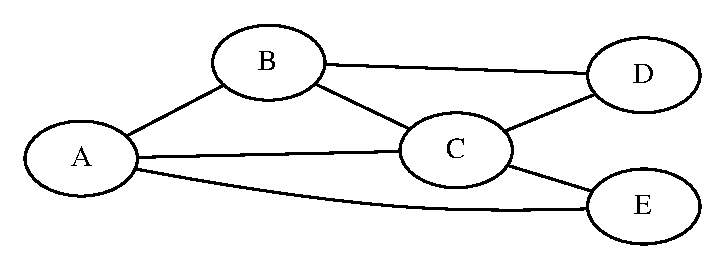
\includegraphics[scale=0.4]{graph2.eps}
			      \end{center}
			      \begin{itemize}
				      \item<2-> Donner les voisins de $A$
				      \item<3-> Donner le degré de $B$
				      \item<4-> Ce graphe est-il orienté ? est-il complet ? est-il simple ?
				      \item<5-> Donner une chaine de longueur 3 dans ce graphe.
			      \end{itemize}
			\item<6-> Dessiner un graphe complet ayant 5 sommets, combien d'arêtes possède ce graphe ?
			\item<7-> Dessiner tous les graphes non orientés ayant 3 sommets.
		\end{enumerate}
	\end{exampleblock}
\end{frame}

% Implémentation des graphes par matrice d'adjacence
\begin{frame}
	\mframe{\GR}
	\begin{alertblock}{Représentation par matrice d'adjacence}
		On peut représenter un graphe à $n$ sommets par sa \textcolor{blue}{matrice d'adjacence} $M$, c'est à dire un tableau de $n$ lignes et $n$ colonnes :
		\begin{itemize}
			\item<2-> On numérote les sommets du graphe
			\item<3-> S'il y a une arête du sommet $i$ vers le sommet $j$ alors on place un 1 à la ligne $i$ et à la colonne $j$ de $M$
			\item<4-> Sinon on place un 0
		\end{itemize}
	\end{alertblock}
	\begin{block}{Remarques}
		\begin{itemize}
			\item<5-> Si le graphe n'est pas orienté alors la matrice est symétrique par rapport à sa première diagonale.
			\item<6-> On peut representer les graphes pondérés en écrivant le poids à la place du 1 pour chaque arête.
		\end{itemize}
	\end{block}
\end{frame}

% Exemple de matrice d'adjacences
\begin{frame}
	\mframe{\GR}
	\begin{exampleblock}{Exemple}
		\begin{enumerate}
			\item<1-> En supposant les sommets numérotés dans l'ordre alphabétique, écrire la matrice d'adjacence du graphe suivant :
			      \begin{center}
				      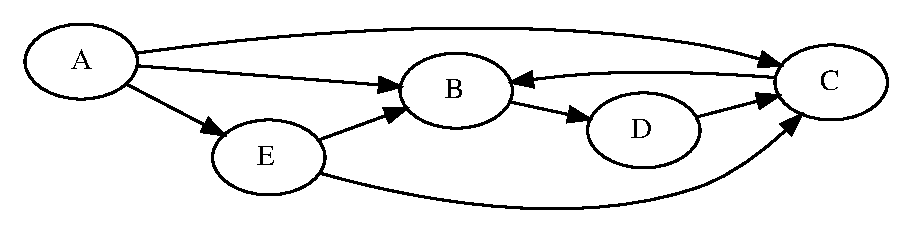
\includegraphics[scale=0.5]{graph3.eps}
			      \end{center}
			\item<2-> Dessiner le graphe ayant la matrice d'adjacence suivante (on appellera les sommets $S_1, S_2, \dots $) :\\
			      $\begin{pmatrix}
					      0 & 0 & 1 & 1 & 1 \\
					      1 & 0 & 1 & 0 & 0 \\
					      1 & 1 & 0 & 0 & 1 \\
					      1 & 0 & 0 & 1 & 0 \\
					      0 & 0 & 1 & 0 & 0 \\
				      \end{pmatrix}$
		\end{enumerate}
	\end{exampleblock}
\end{frame}


% Implémentation des graphes par liste d'adjacence
\begin{frame}
	\mframe{\GR}
	\begin{alertblock}{Représentation par listes d'adjacence}
		On peut représenter un graphe à l'aide de listes d'adjacences, c'est à dire en mémorisant pour chaque sommet du graphe la liste de ses voisins.
		\begin{itemize}
			\item<2-> On crée pour chaque sommet du graphe une liste
			\item<3-> S'il y a une arête du sommet $S_i$ vers le sommet $S_j$ alors  $S_j$ est dans la liste de $S_i$
		\end{itemize}
	\end{alertblock}
	\begin{block}{Remarques}
		\begin{itemize}
			\item<5-> Lorsqu'un graphe a "peu" d'arête cette implémentation est plus intéressante en terme d'occupation mémoire que celle par matrice d'adjacence.
			\item<6-> En Python, on utilisera un dictionnaire pour représenter les listes d'adjacences, les clés sont les sommets et les valeurs les listes associées
		\end{itemize}
	\end{block}
\end{frame}

% Exemple de liste d'adjacences
\begin{frame}[fragile]
	\mframe{\GR}
	\begin{exampleblock}{Exemple}
		\begin{enumerate}
			\item<1-> Ecrire les listes d'adjacences du graphe suivante :
			      \begin{center}
				      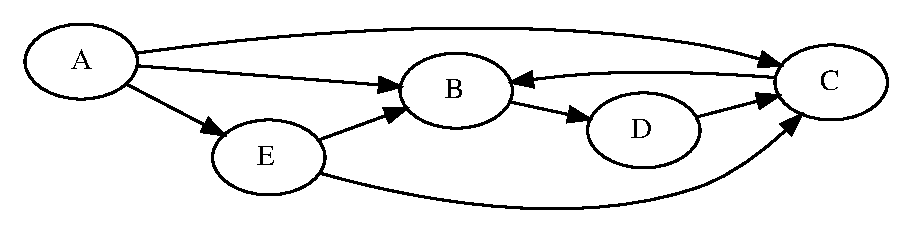
\includegraphics[scale=0.5]{graph3.eps}
			      \end{center}
			\item<2-> Dessiner le graphe représenté par le dictionnaire Python suivante :
			      \begin{lstlisting}
{ 	
	'A' : ['C'],
 	'B' : ['D','E'],
 	'C' : ['A','B'],
 	'D' : ['A','C'],
 	'E' : ['B','C','D']
} 
\end{lstlisting}
		\end{enumerate}
	\end{exampleblock}
\end{frame}

% Exemple de matrice d'adjacences
\begin{frame}
	\mframe{\GR}
	\begin{block}{Parcours d'un graphe}
		De la même façon que pour les arbres, un graphe peut être parcouru de plusieurs façons :
		\begin{itemize}
			\item<1-> dans un \textcolor{blue}{parcours en profondeur}, consiste à passer par le premier voisin non encore parcouru à chaque étape.
			\item<2-> dans un \textcolor{blue}{parcours en largeur}, consiste à parcourir les voisins immédiats, puis les voisins des voisins, etc ...
		\end{itemize}
	\end{block}
	\onslide<3->{
	\begin{exampleblock}{Exemple}
		\begin{center}
			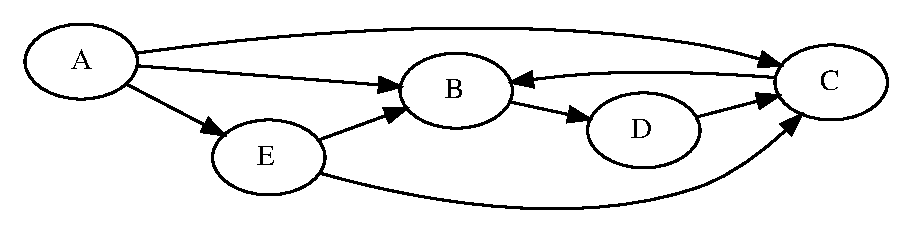
\includegraphics[scale=0.5]{graph3.eps}
		\end{center}
		\begin{itemize}
			\item<4-> En profondeur : \onslide<5->{\textcolor{OliveGreen}{A, B, D, C, E}}.
			\item<6-> En largeur : \onslide<7->{\textcolor{OliveGreen}{A, B, E, D, C}}.
		\end{itemize}
	\end{exampleblock}}
\end{frame}


\end{document}